\section{Experiments}\label{sec:experiments}
We evaluate preference-based alignment, mathematical and logical reasoning, and multi-step tool use with OpenRLHF~\citep{hu2024openrlhf}. The basic variant is used in the alignment and reasoning experiments; \baseline is used in the tool-use comparison. All reported losses use a mean over valid tokens within each response followed by a mean over responses (\cref{appendix:batch_mean}).

\subsection{Preference-based alignment}\label{sec:alignment}
\paragraph{Setup.}
We train a Llama-3-8B-SFT policy on 20,000 prompts using a Bradley--Terry reward model trained on approximately 700,000 human-preference pairs. We compare \ours with one sampled response per prompt against GRPO and RLOO with four responses per prompt, and ReMax with one sampled and one greedy response. Evaluation uses Arena-Hard~\citep{li2024crowdsourced}.

\begin{table}[htbp]
\caption{Arena-Hard results. Length is the mean generated response length, and score/length is their ratio. REINFORCE++ achieves a competitive score with one sampled response per prompt.}
\label{tab:alignment}
\centering
\begin{tabular}{lrrr}
\toprule
Method & Score & Length & Score/length \\
\midrule
\ours ($k=1$) & 46.7 & 832 & \textbf{0.0561} \\
GRPO ($k=4$) & \textbf{46.8} & 860 & 0.0544 \\
RLOO ($k=4$) & 44.6 & 866 & 0.0515 \\
ReMax (1 sampled + 1 greedy) & 45.1 & \textbf{805} & 0.0560 \\
\bottomrule
\end{tabular}
\end{table}

\paragraph{Results.}
\Cref{tab:alignment} shows that \ours obtains 46.7, close to GRPO's 46.8, while generating shorter responses on average (832 versus 860 tokens). It also has the highest score/length ratio among the compared methods. These results demonstrate competitive preference alignment with one sampled response per prompt, enabling the rollout budget to cover a broader set of prompts.

\begin{figure}[htbp]
\centering
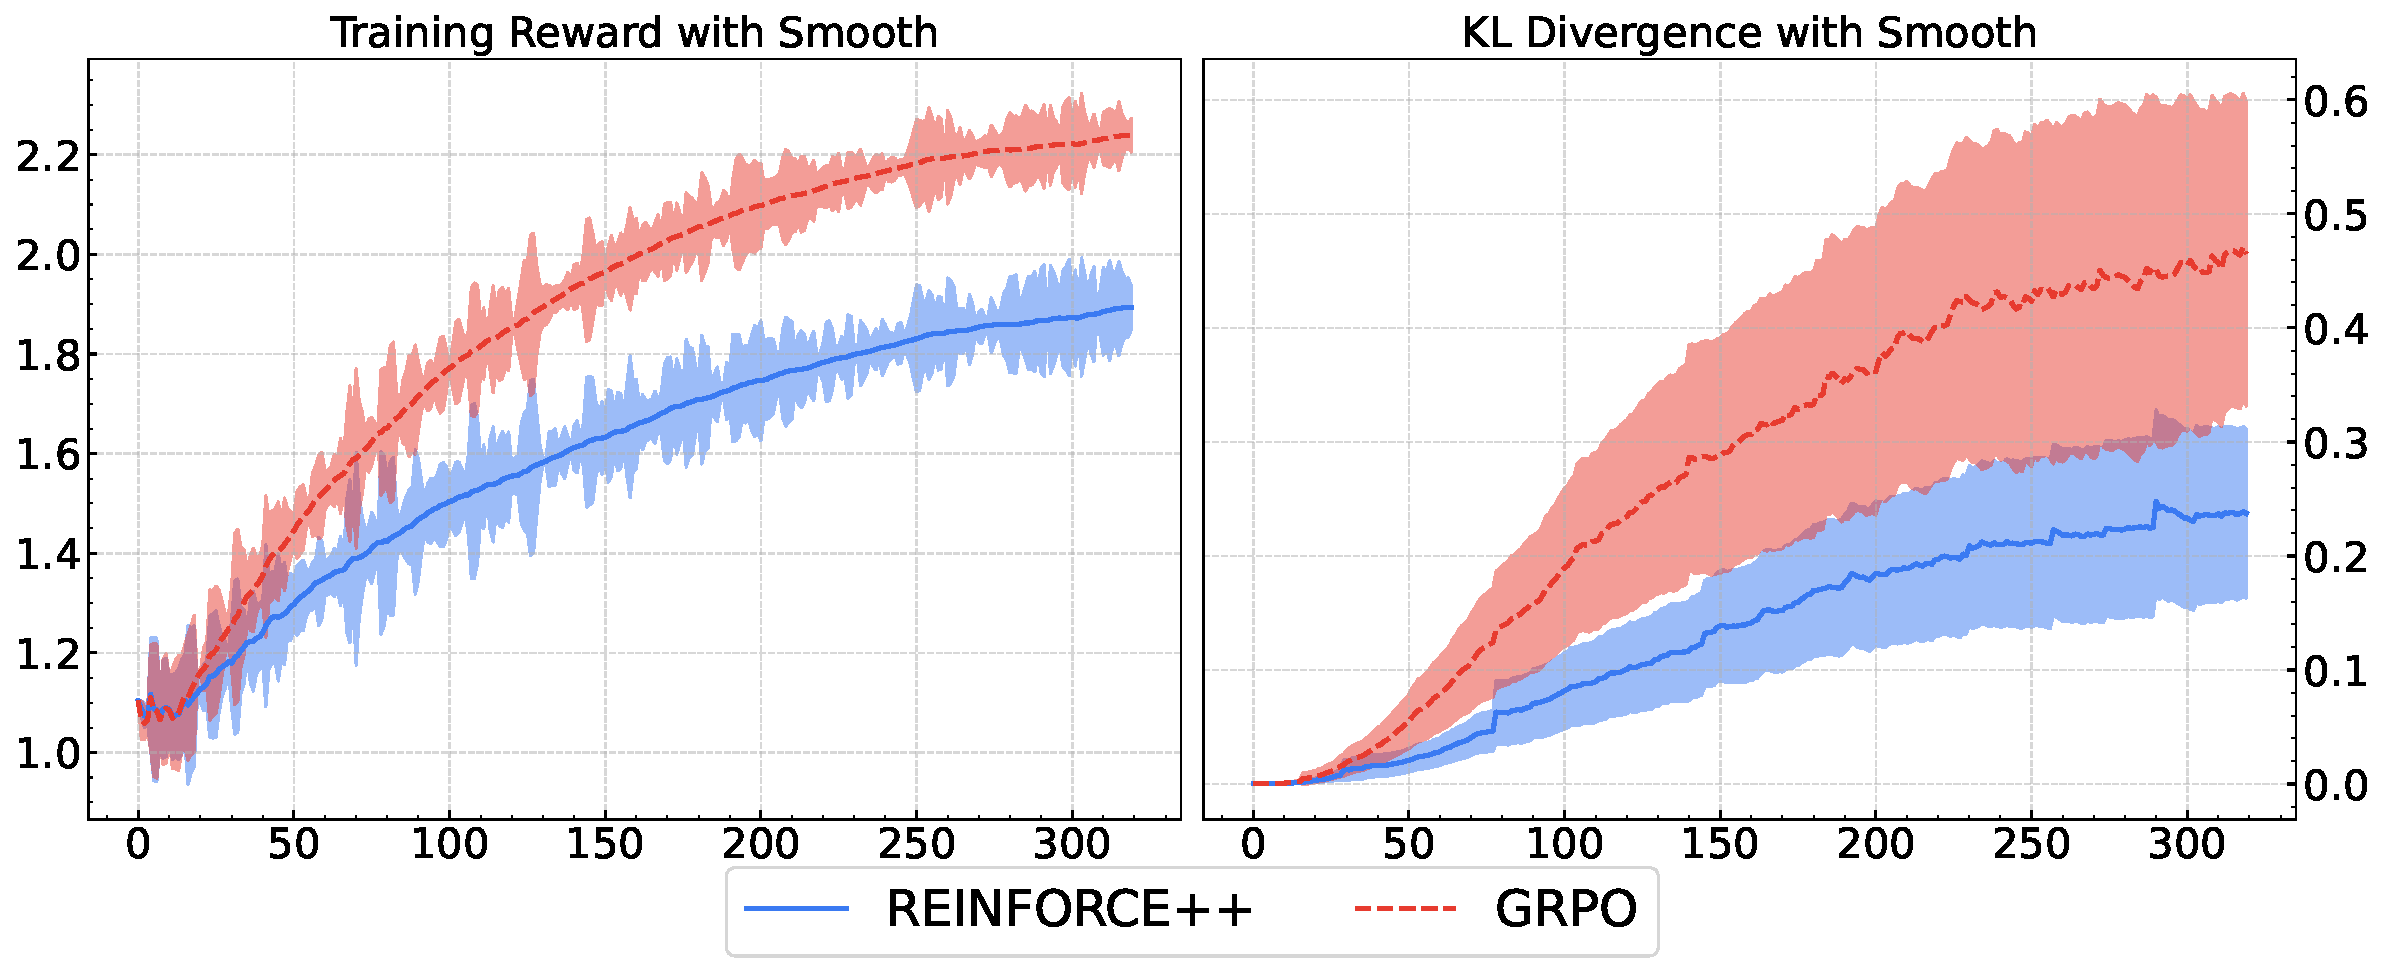
\includegraphics[width=\linewidth]{imgs/orm_reward_kl.pdf}
\caption{Smoothed training reward and KL divergence in preference-based alignment. \ours combines increasing reward with a lower KL divergence throughout the reported training trajectory.}
\label{fig:reward_kl}
\end{figure}

\Cref{fig:reward_kl} shows different reward--KL trade-offs: GRPO's reward rises rapidly alongside its KL divergence, whereas \ours maintains a smaller divergence. This behavior illustrates controlled policy updates under global normalization and KL-regularized returns.

\FloatBarrier
\subsection{Mathematical and logical reasoning}\label{sec:reasoning}
These experiments use the basic \ours variant with grouped sampling ($k>1$) and compare it with GRPO. Mathematical reasoning is trained with verifiable rewards, following the broader RLVR setting~\citep{guo2025deepseek,seed2025seed1}.

\paragraph{Learning from a small prompt set.}
We train on 30 AIME 2024 questions and evaluate on AIME 2025. In \cref{tab:small}, GRPO has the higher training score (95.0 versus 71.0), while \ours has the higher held-out scores: 2.5 versus 0.0 at pass@1 and 40.0 versus 0.4 at pass@16. The comparison highlights the distinction between fitting the training prompts and transferring to a new problem set. In this small-data setting, global normalization is associated with stronger held-out performance.

\begin{table}[htbp]
\caption{Small-data reasoning results, reported in percent. Training uses 30 AIME 2024 questions; held-out evaluation uses AIME 2025.}
\label{tab:small}
\centering
\begin{tabular}{lrrr}
\toprule
 & AIME 2024 (train) & \multicolumn{2}{c}{AIME 2025 (test)} \\
\cmidrule(lr){3-4}
Method & pass@1 & pass@1 & pass@16 \\
\midrule
GRPO & \textbf{95.0} & 0.0 & 0.4 \\
\ours ($k>1$) & 71.0 & \textbf{2.5} & \textbf{40.0} \\
\bottomrule
\end{tabular}
\end{table}

The prompt-level training traces in \cref{appendix:curves} show rapid saturation for many GRPO trajectories and a more gradual progression for \ours. Together with the held-out results, these traces illustrate distinct learning dynamics in the small-data regime.



\paragraph{Knights and Knaves puzzles.}
We evaluate logical reasoning using Knights and Knaves puzzles~\citep{xie2025logic,xie2024memorization}, with difficulty indexed by the number of people in each puzzle. \Cref{fig:logic} shows that GRPO is competitive on the two- and three-person tasks, while \ours scores higher for tasks with four or more people. The reported mean score is 62.1 for \ours and 55.7 for GRPO. The advantage on larger puzzles suggests better transfer across the evaluated difficulty levels.

\begin{figure}[htbp]
\centering
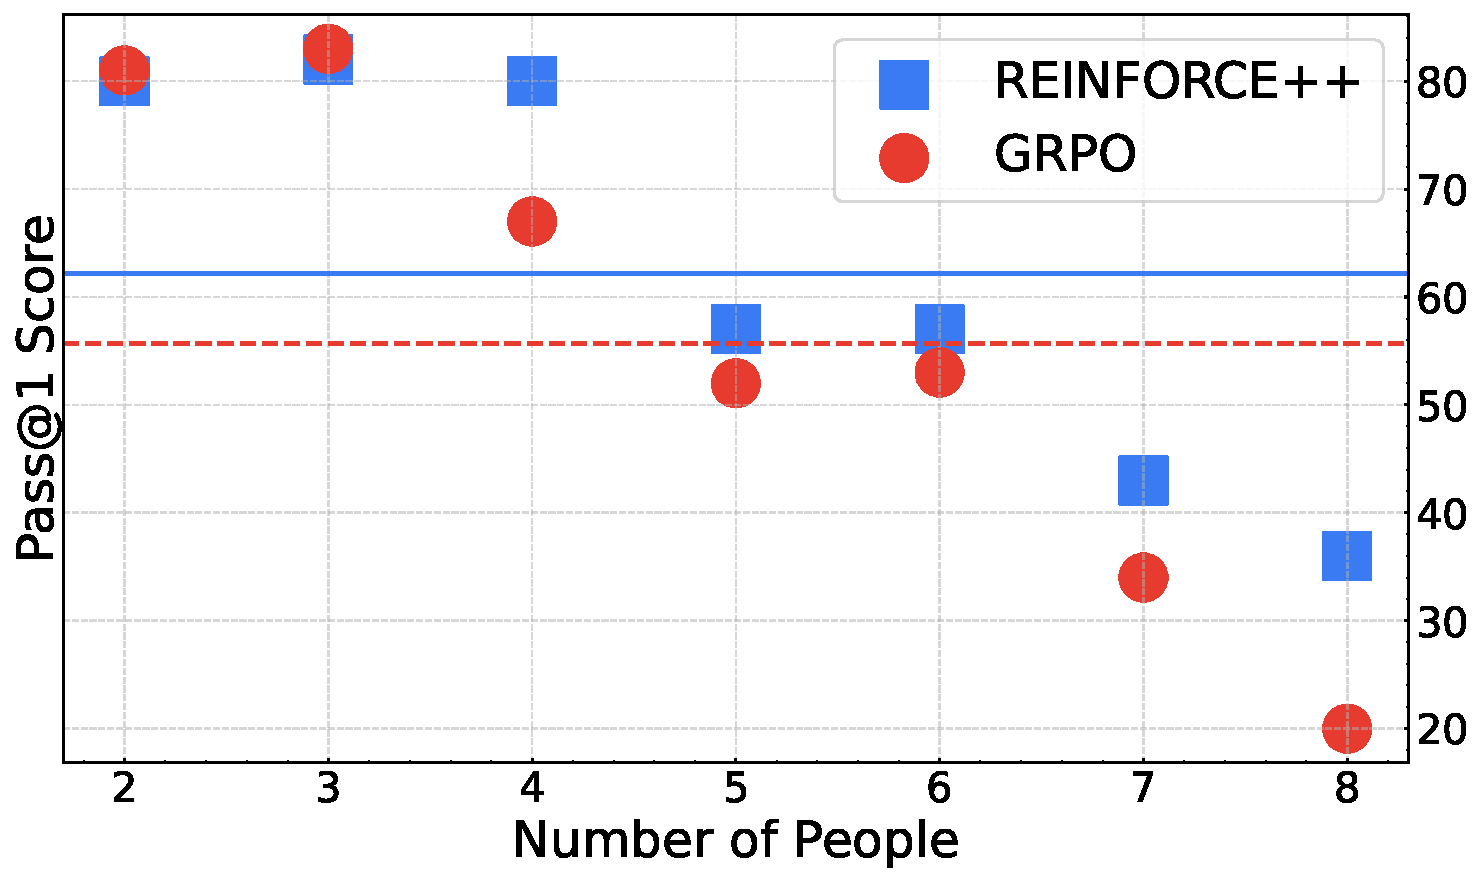
\includegraphics[width=0.76\linewidth]{imgs/logic_score.pdf}
\caption{Knights and Knaves results as the number of people increases. \ours scores higher on the evaluated tasks with at least four people, including the eight-person out-of-distribution setting.}
\label{fig:logic}
\end{figure}

\paragraph{RL from a base model.}
We also apply RL directly to a Qwen2.5-Math-Base model on MATH dataset splits. \Cref{tab:zero} reports higher scores for \ours on both out-of-distribution benchmarks: 21.04 versus 18.96 on AIME 2024 and 60.47 versus 59.22 on AMC 2023. Its MATH-500 score remains close to GRPO's (72.00 versus 73.00), extending the generalization results to RL initialized from a base model.

\begin{table}[htbp]
\caption{Reasoning results after RL from Qwen2.5-Math-Base. OOD and ID denote out-of-distribution and in-distribution evaluation relative to the training task. Scores are percentages.}
\label{tab:zero}
\centering
\begin{tabular}{lrrr}
\toprule
 & AIME 2024 (OOD) & AMC 2023 (OOD) & MATH-500 (ID) \\
Method & pass@8 & pass@8 & pass@1 \\
\midrule
GRPO & 18.96 & 59.22 & \textbf{73.00} \\
\ours & \textbf{21.04} & \textbf{60.47} & 72.00 \\
\bottomrule
\end{tabular}
\end{table}

\FloatBarrier
\subsection{Multi-step tool use}\label{sec:tools}
\paragraph{Setup.}
We use the ZeroTIR environment and its training and evaluation protocol~\citep{mai2025agentrlscalinglaw}. A Qwen2.5-7B base policy learns to call Python tools to solve mathematical problems. Training uses OpenRLHF and data from ORZ~\citep{hu2025openreasonerzeroopensourceapproach} and DAPO~\citep{yu2025dapoopensourcellmreinforcement}. Evaluation covers AIME 2024, AIME 2025, HMMT February 2024 and 2025, and CMIMC, using average@32. This metric averages success over 32 sampled attempts rather than counting success if any one attempt is correct.

\begin{table}[htbp]
\caption{Multi-step tool-use scores (average@32, in percent). ``Baseline'' denotes \baseline. The last column is the unweighted mean across the five benchmarks.}
\label{tab:tools}
\centering
\small
\begin{tabular}{lrrrrrr}
\toprule
 & \multicolumn{2}{c}{AIME} & \multicolumn{2}{c}{HMMT Feb.} & & \\
\cmidrule(lr){2-3}\cmidrule(lr){4-5}
Method & 2024 & 2025 & 2025 & 2024 & CMIMC & Mean \\
\midrule
GRPO & \textbf{31.66} & 21.87 & 16.97 & 17.70 & 24.68 & 22.58 \\
PPO & 30.20 & 21.66 & 15.00 & 18.43 & 23.95 & 21.85 \\
Baseline & 30.83 & \textbf{27.18} & \textbf{17.91} & \textbf{18.95} & \textbf{25.62} & \textbf{24.10} \\
\bottomrule
\end{tabular}
\end{table}

\paragraph{Results.}
\baseline obtains the highest mean score, 24.10, compared with 22.58 for GRPO and 21.85 for PPO (\cref{tab:tools}). It leads on four of the five benchmarks. The absolute mean improvements are 1.52 and 2.25 percentage points over GRPO and PPO, respectively. The largest gain over GRPO occurs on AIME 2025, where the score increases from 21.87 to 27.18. These results demonstrate the effectiveness of the combined training recipe for multi-step tool use.
